\section{Observation and Calculations}
\subsection{Monoatomic Lattice}
The experimentally obtained data for the monotomic
lattice is shown in Table \ref{tab:mono1}. The phase difference was observed using the oscilloscope in XY mode, with one input being from the signal generator and the other from the LC circuit output. Measurements were taken at every phase change of $\pi/2$ where the oscilloscope display switched between an ellipse (phase difference $\pm \pi/2$; Fig. \ref{tk1}) and a straight line (phase difference 0 or $\pi$; Fig. \ref{tk2}).

\begin{figure}[H]
    \centering
    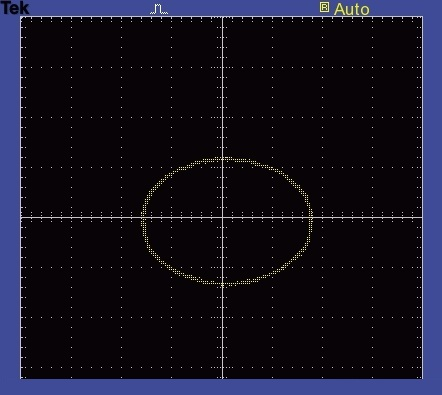
\includegraphics[width=.8\columnwidth]{images/TEK0000.JPG}
    \caption{Oscilloscope output in XY mode showing a phase difference $\pm \pi/2$}
    \label{tk1}
\end{figure}

\begin{figure}[H]
    \centering
    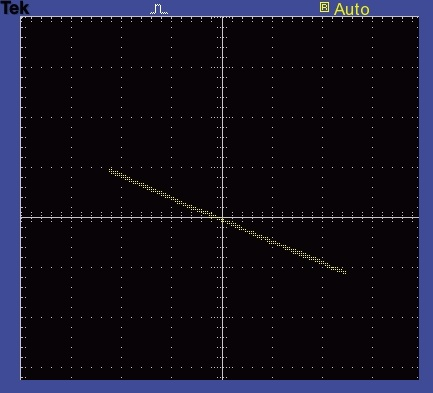
\includegraphics[width=.8\columnwidth]{images/TEK0001.JPG}
    \caption{Oscilloscope output in XY mode showing a phase difference 0 or $\pi$}
    \label{tk2}
\end{figure}

The corresponding inductance and capacitance values used are given in Table \ref{tab:mono}. The graph of $\theta$ vs $f$ for the monoatomic lattice is shown in Fig. \ref{g1}.
\begin{table}[]
    \centering
    \begin{tabular}{|c|c|c|}
    \hline
    S.No. & L (mH) & C (nF) \\ \hline
    1 & 0.993 & 48.52 \\ 
    2 & 0.981 & 48.88 \\ 
    3 & 0.965 & 48.06 \\ 
    4 & 0.982 & 50.15 \\ 
    5 & 0.959 & 48.33 \\ 
    6 & 0.965 & 50.75 \\ 
    7 & 0.978 & 49.93 \\ 
    8 & 0.992 & 47.19 \\ 
    9 & 0.980 & 48.01 \\ 
    10 & 0.967 & 47.39 \\ \hline
    Mean & 0.976 & 48.721 \\ \hline
    Std. Dev. & 0.011 & 1.136 \\ \hline
    \end{tabular}
    \caption{Measured values of the component of the circuit for a monoatomic lattice}
    \label{tab:mono}
    \end{table}
\begin{table}[]
    \centering
    \begin{tabular}{|c|c|c|c|}
    \hline
    Total phase & Phase change & Frequency & $\omega$ \\
    Change  ($^\circ$) & per unit cell ($^\circ$) & (Hz) & (krad /s) \\ \hline
    90 & 9 & 2.151 & 13.52 \\ 
    180 & 18 & 6.771 & 42.54 \\ 
    270 & 27 & 10.250 & 64.40 \\ 
    360 & 36 & 13.870 & 87.15 \\ 
    450 & 45 & 17.100 & 107.44 \\ 
    540 & 54 & 20.580 & 129.31 \\ 
    630 & 63 & 23.740 & 149.16 \\ 
    720 & 72 & 27.210 & 170.97 \\ 
    810 & 81 & 30.270 & 190.19 \\ 
    900 & 90 & 33.300 & 209.23 \\ 
    990 & 99 & 36.030 & 226.38 \\ 
    1080 & 108 & 38.830 & 243.98 \\ 
    1170 & 117 & 41.270 & 259.31 \\ 
    1260 & 126 & 43.410 & 272.75 \\ 
    1350 & 135 & 45.300 & 284.63 \\ 
    1440 & 144 & 47.130 & 296.13 \\ 
    1530 & 153 & 48.730 & 306.18 \\ 
    1620 & 162 & 50.680 & 318.43 \\ \hline
    \end{tabular}
    \caption{Observed frequenciesand their corresponding phase changes in the circuit for a monoatomic lattice}
    \label{tab:mono1}
\end{table}

\begin{figure}
    \centering
    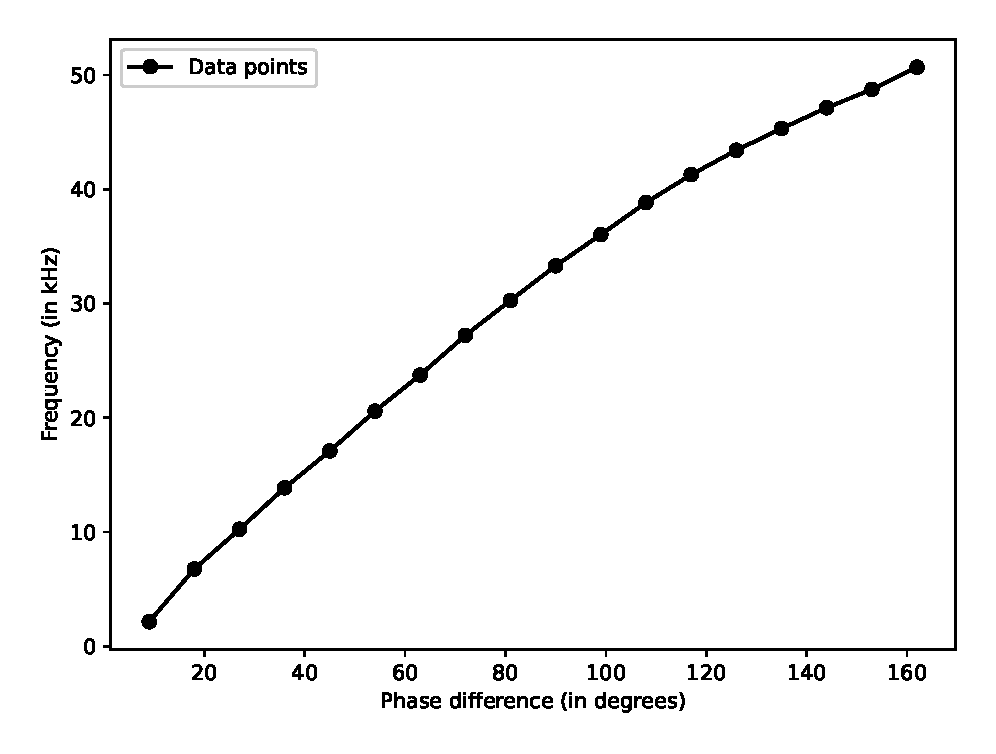
\includegraphics[width=1\columnwidth]{images/mono.eps}
    \caption{Plot showing $\theta$ vs. $f$ for the monoatomic lattice}
    \label{g1}
\end{figure}

Now, using Eq. \ref{wf}, the theoretical value of $\omega_\text{max}$ can be calculated from the measured average values of $L$ and $C$ as,

\begin{align*}
    \omega_\text{max} &= \frac{2}{\sqrt{0.976 \times 10^{-3} \times 48.72 \times 10^{-9}}}\\ &= 290.00 \text{ krad/s}\\ \text{or, }f_\text{max} &= 46.16 \text{ kHz}
\end{align*}

From the experimental, the maximum frequency observed is 50.68 kHz or 318.43 krad/s.

\subsection{Diatomic Lattice}
The experimentally obtained data for the diatomic
lattice is shown in Table \ref{tab:di1}. The corresponding inductance and capacitance values used are given in Table \ref{tab:di}. The graph of $\theta$ vs $f$ for the diatomic lattice is shown in Fig. \ref{g1}.
\begin{table}[]
    \centering
    \begin{tabular}{|c|c|c|c|}
    \hline
    S.No. & L (mH) & $C_1$ (nF) & $C_2$ (nF) \\ \hline
    1 & 0.993 & 48.52 & 157.18 \\ 
    2 & 0.981 & 48.88 & 152.36 \\ 
    3 & 0.965 & 48.06 & 152.20 \\ 
    4 & 0.982 & 50.15 & 148.54 \\ 
    5 & 0.959 & 48.33 & 150.74 \\ 
    6 & 0.965 &  &  \\ 
    7 & 0.978 &  &  \\ 
    8 & 0.992 &  &  \\ 
    9 & 0.980 &  &  \\ 
    10 & 0.967 &  &  \\ \hline
    Mean & 0.976 & 48.570 & 152.20 \\ \hline
    Std. Dev. & 0.011 & 0.705 & 2.84 \\ \hline
    \end{tabular}
    \caption{Measured values of the component of the circuit for a diatomic lattice}
    \label{tab:di}
\end{table}
\begin{table}[]
    \centering
    \begin{tabular}{|c|c|c|c|}
    \hline
    Total phase & Phase change & Frequency & $\omega$ \\
    Change  ($^\circ$) & per unit cell ($^\circ$) & (Hz) & (krad /s) \\ \hline
    90 & 9 & 2.160 & 13.57 \\ 
    180 & 18 & 4.725 & 29.69 \\ 
    270 & 27 & 7.247 & 45.53 \\ 
    360 & 36 & 9.715 & 61.04 \\ 
    450 & 45 & 12.030 & 75.59 \\ 
    540 & 54 & 14.300 & 89.85 \\ 
    630 & 63 & 16.330 & 102.60 \\ 
    720 & 72 & 18.140 & 113.98 \\ 
    810 & 81 & 20.130 & 126.48 \\ 
    900 & 90 & 25.220 & 158.46 \\ 
    990 & 99 & 28.310 & 177.88 \\ 
    1080 & 108 & 31.950 & 200.75 \\ 
    1170 & 117 & 34.900 & 219.28 \\ 
    1260 & 126 & 36.470 & 229.15 \\ 
    1350 & 135 & 37.680 & 236.75 \\ 
    1440 & 144 & 38.820 & 243.91 \\ 
    1530 & 153 & 40.030 & 251.52 \\ \hline
    \end{tabular}
    \caption{Observed frequencies and their corresponding phase changes in the circuit for a diatomic lattice}
    \label{tab:di1}
\end{table}

\begin{figure}
    \centering
    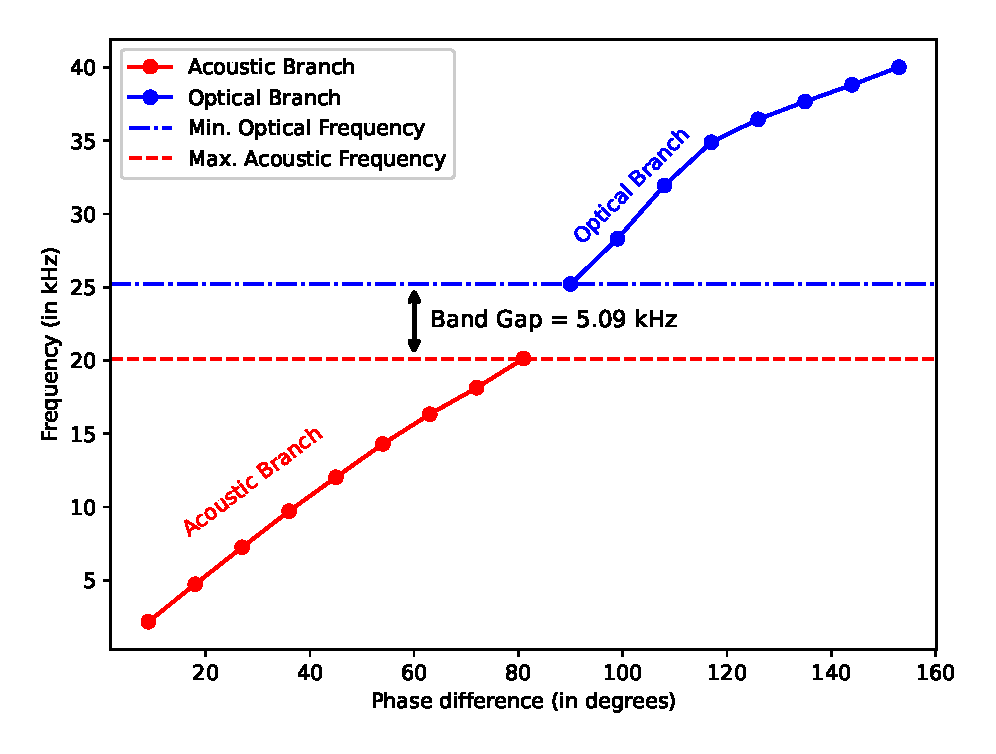
\includegraphics[width=1\columnwidth]{images/di.eps}
    \caption{Plot showing $\theta$ vs. $f$ for the diatomic lattice}
    \label{g2}
\end{figure}

Again, using Eq. \ref{wf2}, the calculated band gap value is,

\begin{align*}
    f_\text{gap} &= \frac{1}{2\pi}\sqrt{\frac{2}{LC_1}} - \frac{1}{2\pi}\sqrt{\frac{2}{LC_2}}\\
    &= 32.79 - 18.52 \\&= 14.27 \text{ kHz}
\end{align*}

From Fig. \ref{g2}, we can see than the lowest frequency in the optical branch is 25.22 kHz and the highest frequency in the acoustic branch is 20.13 kHz. Hence, the experiment band gap is 5.09 kHz.

\section{Error Analysis}

Based on Eq. \ref{wf}, the error in $f_\text{max}$ for the monoatomic lattice can be calculated using

\begin{align}
    \Delta f_\text{max} = f_\text{max}\sqrt{\left(\frac{\Delta L}{2L}\right)^2 + \left(\frac{\Delta C}{2C}\right)^2}
\end{align}

Using the values of standard deviation in the above equation, the error comes out to be $\Delta f_\text{max} = 0.60$ kHz.

Similarly using the above equation for the diatomic lattice, the individual errors in the maximum acoustic and minimum optical frequencies amount to the final error in $\Delta f_\text{max}$,

\begin{align*}
    \Delta f_\text{gap} &= |\Delta f_\text{acoustic, max}| + |\Delta f_\text{optical, min}|\\
    &= 0.03 + 0.02 \\
    &= 0.05 \text{ kHz}
\end{align*}